
\chapter{Estado del Arte}

    \noindent En esta sección nuestro objetivo será realizar una investigación por la literatura y los artículos publicados relacionados con el reconocimiento automático de landmarks cefalométricos en tareas de antropología forense para finalmente justificar nuestra elección en el presente trabajo para tratar de resolver el problema. Para ello utilizaremos la base de datos \textit{Scopus} para realizar la búsqueda y consulta de artículos científico publicados.

    \section{Localización de landmarks cefalométricos en imágenes}

        \noindent Para hacernos una primera idea del estado actual del problema de reconocimiento de landmarks faciales en imágenes realizamos una primera consulta en \textit{SCOPUS} (\autoref{fig:SCOPUS1}) con la siguiente \textit{keyword} restringiendo los artículos a aquellos relacionados con la informática:
        
        \begin{verbatim}
            TITLE-ABS-KEY ( 
                facial  
                AND  
                ( landmarks  OR  keypoints )  
                AND  
                detection 
                )  
                AND  
                ( LIMIT-TO ( SUBJAREA ,  "COMP" ) )
        \end{verbatim}
        
        \medskip
        
        \noindent Como podemos observar, actualmente existe una tendencia creciente en la publicación de papers relacionados con este tema, en particular esta tendencia comienza en los años en que surge el Deep Learning y las CNN comienzan a utilizarse en visión por computador para el tratamiento de imágenes. 

        \begin{figure}[htpb]
            \centering
            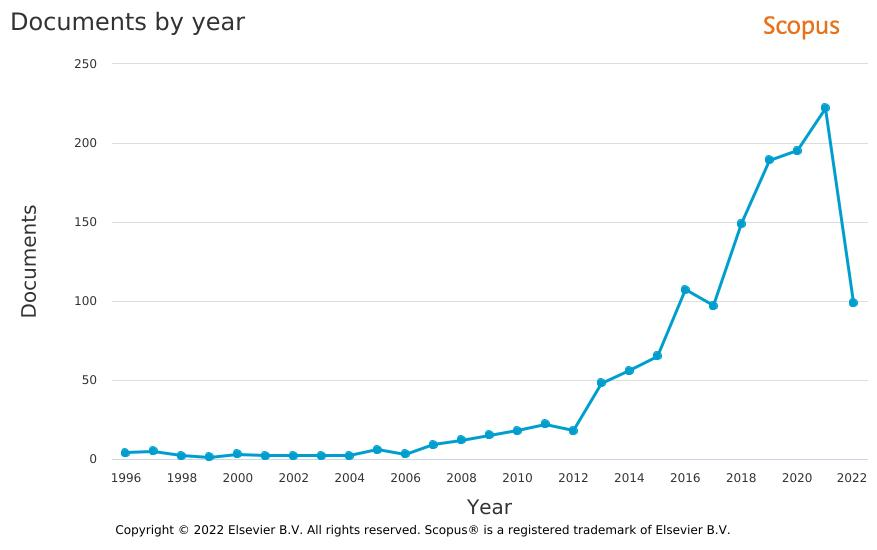
\includegraphics[width=0.6\textwidth]{img/Scopus_1.jpg}
            \caption{Gráfica de publicaciones por año obtenida con la primera \textit{keyword} el $14$ de Julio de $2022$. Destaca el notable incremento de papers a partir de 2012, año en que aparece la red AlexNet y comienza a ganar popularidad el Deep Learning en el tratamiento de imágenes.}
            \label{fig:SCOPUS1}
        \end{figure}

        \medskip

        \noindent Sin embargo los artículos que se han encontrado en la \autoref{fig:SCOPUS1} no guardan una relación muy estrecha con el problema de deteción de landmarks cefalométricos en problemas de antropología forense, por ello para descubrir el estado del arte en este campo nos vemos obligados a realizar otra consulta en scopus un poco más concreta y que nos permita conocer mejor las publicaciones más relevantes en este campo en los últimos años descartando los que no sean artículos relacionados con informática. La consulta que realizamos es la siguiente: 

        \begin{verbatim}
            TITLE-ABS-KEY ( 
                ( 
                    ( anthropology  OR  ( anthropology  AND  forensic ) )  
                    AND  
                    ( cephalometric  AND  ( landmarks  OR  keypoints ) ) 
                )  
                
                OR  
                
                ( 
                    ( anthropology  OR  ( anthropology  AND  forensic ) )  
                    AND  
                    ( facial  AND  ( landmarks  OR  keypoints ) ) 
                ) 
                )  
                AND  
                ( LIMIT-TO ( SUBJAREA ,  "COMP" ) )
        \end{verbatim}

        \medskip

        \noindent Con la búsqueda anterior se obtienen un total de $14$ artículos, algo que nos confirma que es un área de investigación en la que apenas hay bibliografía o artículos. Podemos ver un gráfico de resultados de la búsqueda en \autoref{fig:SCOPUS2}.

        \begin{figure}[htpb]
            \centering
            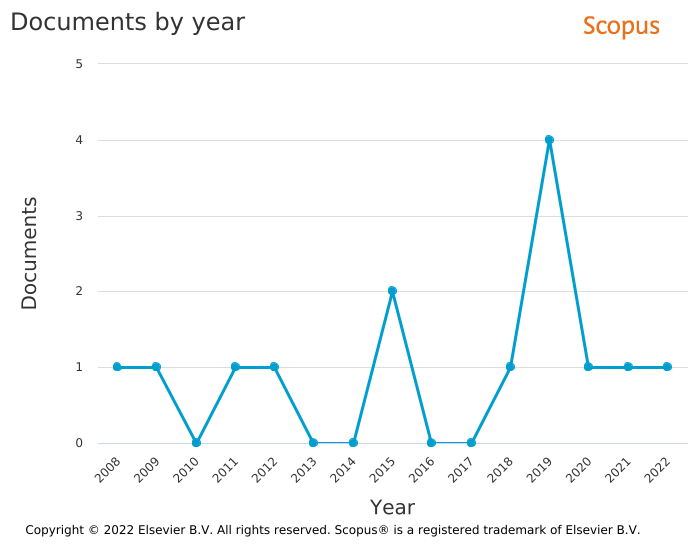
\includegraphics[width=0.6\textwidth]{img/Scopus_2.png}
            \caption{Gráfica de publicaciones por año obtenida con la segunda \textit{keyword} el $14$ de Julio de $2022$. La tendencia es a un artículo por año, aunque destaca el pico de tres artículos en 2015 y el de cuatro en 2019.}
            \label{fig:SCOPUS2}
        \end{figure}

        \subsection{Evolución en la identificación forense de landmarks cefalométricos}
            
            \noindent Como hemos visto antes, la literatura existente es prácticamente nula, además de los catorce artículos obtenidos con la búsqueda anterior, la mayoría no se centran en el reconocimiento de landmarks cefalométricos en imágenes de rostros, hay artículos que se centran en la superposición craneofacial y otros basados en la identificación de landmarks en cráneos. Por lo tanto, de los catorce artículos vamos a destacar los siguientes por la relación directa con nuestro problema ordenados de mayor a menor antigüedad: 

            \subsubsection{Two different approaches to handle landmark location uncertainty in skull-face overlay: coevolution vs fuzzy landmarks}
                \noindent Se trata de un artículo pulicado en $2011$ por Óscar Ibáñez et al \cite{ibanez2011two} en el cual abordan el problema de la superposición craneofacial diseñando un nuevo algoritmo basado en coevolución capaz de reducir el proceso de \textit{Skull-face overlay} (SFO) que tradicionalmente podía llegar a tardar unas 24 horas y comparándolo con un algoritmo ya existente basado en landmarks imprecisos en el cual el antropólogo forense marca regiones de la imagen en las que se encuentra cada landmark (esta tarea no está automatizada en este algoritmo). Aunque no guarda una relación directa con el problema, el algoritmo propuesto realiza una identificación de landmarks cefalométricos en imágenes, por lo que hemos decidido incluirlo en el estudio.

                \medskip

                \noindent Durante el proceso de SFO se dispone de un modelo $3$D de un cráneo y de una imagen, de manera que se considera exitoso el proceso cuando se coloca el cráneo en la misma posición en que aparece en la imagen. Durante este proceso se deben tener en cuenta factores como la edad de la persona, el peso o las expresiones faciales, que añaden un grado más de dificultad a la tarea.

                \medskip

                \noindent Generalmente se dispone de un conjunto de landmarks marcados tanto en la imagen como en el cráneo, y la tarea del SFO se reduce en calcular la transformación que permite llevar los landmarks del cráneo a ocupar la misma posición que en la imagen.

                \medskip

                \noindent La alternativa al algoritmo basado en landmarks imprecisos es un algorimto coevolutivo en el cual el valor de la función de fitness de cada elemento depende de la de él mismo y otros individuos que pueden interaccionar de forma cooperativa o conflictiva. Adaptado al problema de SFO tendríamos dos poblaciones: el conjunto de parámetros que definen la transformación que se aplica al modelo $3$D del cráneo y por otro lado las localizaciones de los landmarks cefalométricos. Ambas poblaciones colaboran para encontrar la mejor transformación posible y solucionar el SFO.

                \medskip

                \noindent En el experimento se disponía de seis procesos distintos de SFO correspondientes a tres casos reales proporcionados por el laboratorio de Antropología Física de la Universidad de Granada en colaboración con la policía científica. Se disponía así de tres modelos $3$D de cráneos pertenecientes a personas desaparecidas junto con un dataset de seis imágenes. Las imágenes, a pesar de ser pocas, presentan una gran variedad en iluminación, posición (hay imágenes frontales y en $3/4$) y con problemas de oclusión en algunos casos para los landmarks a causa del cabello. Por otro lado la calidad de las imágenes es muy variada, habiendo imágenes de gran resolución y otras de baja calidad. Finalmente se disponen cuatro imágenes para el caso de estudio $3$ y una única imagen para el caso de estudio $1$ y $2$.

                \medskip
                

                \noindent En el experimento, el algoritmo empleado para la técnica de encontrar landmarks imprecisos es CMA-ES, y se comparó con el algoritmo coevolutivo desarrollado. Las conclusiones fueron que el nuevo algoritmo reducía considerablemente los tiempos de ejecución del algoritmo basado en landmarks imprecisos y que realizaba una Localización de landmarks cefalométricos apropiada. 
                
                \medskip

                \noindent Por lo tanto podemos considerar este primer algoritmo coevolutivo como la primera aproximación a nuestro problema de detección automática de landmarks. A pesar de lo pobre que es el conjunto de datos de entrenamiento, se emplean imágenes que se encuentran en nuestro dataset y con diversas posturas y resolución de imagen. No obstante, la parte de detección de landmarks no es la principal de este artículo, pues aunque es una consecuencia del algoritmo que se desarrolla, se pretende realizar con el mayor éxito posible la fase SFO.

            \subsubsection{Automatic craniofacial anthropometry landmarks detection and measurements for the orbital region}
                \noindent Se trata de un artículo publicado en $2014$ por Salina Mohd et al \cite{asi2014automatic} en el que se pretende diseñar un método para calcular en una imagen de los ojos de un sujeto el \textit{endocathion} y el \textit{exocanthion} basado en el uso de un clasificador entrenado sobre filtros de Haar usados para la identificación de caras por Viola-Jones.

                \medskip

                \noindent Lo primero que llama la atención del artículo es que tan solo pretende ser capaz de identificar dos landmarks, mientras que en nuestro problema por ejemplo tratamos de predecir la posición de unos treinta (incluyendo en \textit{endocathion} y el \textit{exocanthion}).

                \medskip

                \noindent En segundo lugar, cabe destacar la manera en que se resuelve el problema, pues se hace uso de un clasificador en cascada basado en filtros de tipo Haar como se pueden ver en la \autoref{fig:asi2014}. Este es un método tradicional de la visión por computador en el que mediante el paso y convolución de este tipo de filtros por la imagen se obtiene información de esta relativa a los contornos. No obstante se trata de un método que ya se ha visto superado por otras técnicas más recientes de deep learning.

                \begin{figure}[!h]
                    \centering
                    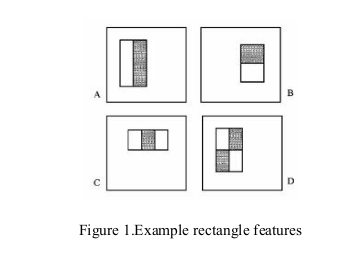
\includegraphics[width=0.8\textwidth]{img/caracteristicas_haar.png}
                    \caption{Ejemplo de filtros empleados en el artículo \cite{asi2014automatic} de donde procede esta imagen.}
                    \label{fig:asi2014}
                \end{figure}

                \medskip

                \noindent Por otro lado, el conjunto de datos que se emplea se ha obtenido en entornos controlados con buena iluminación, algo que no guarda relación con nuestro problema pues se trata de imágenes en diversas posturas, iluminación, y resolución.

            \subsubsection{Automated facial landmark detection, comparison and visualization}
                \noindent Se trata de un trabajo realizado en $2015$ por Marek Galvánek et al. \cite{galvanek2015automated} para la detección automática de landmarks en modelos $3D$ de imágenes de personas. 

                \medskip

                \noindent Los landmarks detectados por el modelo son en total $14$ y todos ellos pertenecen también al conjunto de landmarks que se detectan en este trabajo fin de grado.

                \medskip

                \noindent El algoritmo propuesto se basa en la curvatura de la superficie del modelo $3$D y en la simetría del perfil. En primer lugar se alinea el modelo $3$D con el plano horizontal de Frankfort \autoref{fig:Frankfort}, un plano utilizado por los antropólogos forenses para marcar landmarks. En segundo lugar se realiza un estudio de la curvatura del modelo $3$D en la zona de la nariz, boca y ojos. Finalmente con el perfil del modelo y la simetría se rectifican y perfeccionan los landmarks marcados en etapas previas.

                \begin{figure}[!h]
                    \centering
                    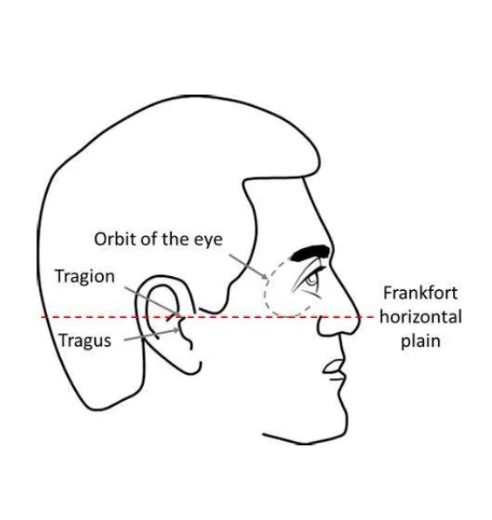
\includegraphics[width=0.5\textwidth]{img/frankfort.png}
                    \caption{Cara alineada con el plano horizontal de Frankfort. Imagen extraida de \url{https://www.slideshare.net/NiharikaSupriya/cephalometrics-landmarkslines-and-planes-93890774
                    }}
                    \label{fig:Frankfort}
                \end{figure}

                \medskip

                \noindent El algoritmo propuesto resulta interesante, aunque no detecta un elevado número de landmarks y se hace de una forma parecida a como un antropólogo forense actuaría. Podemos ver también que es muy preciso en la detección si comparamos los landmarks marcados por el algoritmo con los marcados por un experto manualmente en la \autoref{fig:landmarks_comparativa}.


                \begin{figure}[!h]
                    \centering
                    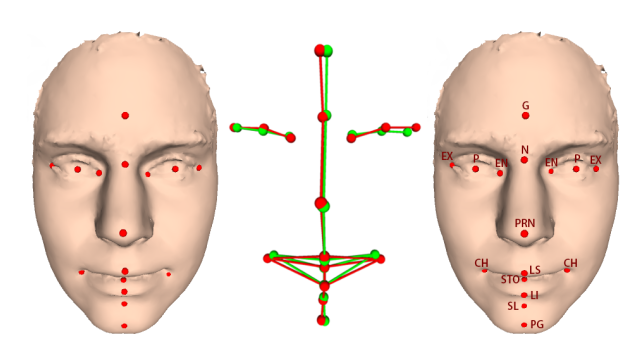
\includegraphics[width=0.8\textwidth]{img/comparativa_landmarks.png}
                    \caption{Comparativa entre los landmarks marcados por el algoritmo (izquierda) y los marcados por un experto (derecha). Imagen extraida de \cite{galvanek2015automated}.}
                    \label{fig:landmarks_comparativa}
                \end{figure}

                \medskip

                \noindent En este trabajo, comenzamos a ver ya un problema similar al nuestro, la detección automática de landmarks cefalométricos con un mayor número de landmarks ($14$ frente a los $2$ del estudio anterior). Aunque se realiza sobte modelos $3$D de caras que evitan problemas de oclusión, mala iluminación o resolución.

            \subsubsection{Automatic cephalometric landmarks detection on frontal faces: An approach based on supervised learning techniques}

                \noindent El siguiente artículo es de $2019$ y fue realizado por Lucas Faria et al. Pretende desarrollar un algoritmo para el reconocimiento automático de landmarks cefalométricos en imágenes frontales a partir de técnicas de visión por computador y de métodos de aprendizaje supervisado \cite{porto2019automatic}.

                \medskip

                \noindent El algoritmo tiene tres componentes:

                \begin{itemize}
                    \item En la primera fase se realiza un pre-procesamiento de las imágenes para resaltar sus caracteristicas faciales. 
                    \item En la segunda fase se aplica la cascada de filtros de Haar de Viola-Jones para identificar las regiones de interés de la imagen: ojos, nariz, boca.
                    \item Finalmente se aplica el algoritmo de machine learning supervisado a cada una de las regiones anteriores. Creando un detector automático de landmarks para cada región.
                \end{itemize}

                \medskip

                \noindent Por otro lado el conjunto de entrenamiento es de $1000$ individuos de los cuales se tomaron fotografías frontales en las mismas condiciones de iluminación y de distancia a la cámara, por lo que no presenta las mismas complicaciones que el dataset del que disponemos. 

                \medskip

                \noindent Destaca este artículo por ser el primero en el cual comienzan a usarse técnicas de aprendizaje automático para la resolución del problema. Además en las imágenes de entrenamiento fueron marcados 28 landmarks que se emplearon para el entrenamiento, que coinciden con los mismos que tenemos en nuestro problema.

            \subsubsection{The Improved Faster R-CNN for Detecting Small Facial Landmarks on Vietnamese Human Face Based on Clinical Diagnosis}
            
                \noindent Este artículo es el más reciente pues fue publicado en Junio de $2022$ por Ho Nguyen Anh Tuan et al \cite{ImprovedfasterRCNN}. En él se utiliza una versión mejorada de la red faster R-CNN aplicada a la tarea del reconocimiento de landmarks cefalométricos. 

                \medskip

                \noindent Los resultados obtenidos son muy buenos pero como ocurre en la mayoría de trabajos de este tipo, la base de datos usada ha sido de imágenes tomadas de voluntarios en unas mismas condiciones de iluminación frontales y de perfil. 

                \medskip

                \noindent No obstante el trabajo restalta la gran importancia que está teniendo el Deep Learning y las CNN en tareas de reconocimiento de landmarks faciales (usualmente landmarks no biológicos como los que se emplean en tareas de antropología forense), y partiendo de esta base podemos justificar el trabajo que vamos a desarrollar, pues nos proponemos adaptar una red que ya ha sido entrenada para la identificación de landmarks faciales en grandes volúmenes de datos de imágenes en diversas posturas y resolución para la tarea del reconocimiento de landmarks forense.

                \medskip

                \noindent Todos los métodos que se han presentado en esta sección trataban de cumplir con el mismo objetivo, y han ido evolucionando con el paso de los años a la par que la informática, empezando por tratar de aplicar algoritmos coevolutivos, después filtros de Haar y técnicas de visión por computador y finalmente usar CNN de Deep Learning. De esta manera y viendo con perspectiva el estado del arte en el campo, consideramos que la propuesta que presentamos puede traer buenos resultados, pues pretendemos enseñar a un sistema experto en el reconocimiento de landmarks no biológicos a identificar estos otros puntos, lo cual puede suponer un nexo de unión entre las dos líneas de investigación.

        \subsection{Nuestra propuesta}
            \noindent El reconocimiento automático de landmarks faciales es una área de gran importancia en la actualidad en tareas como el reconocimiento de personas y que se está viendo muy desarrollado actualmente por la gran capacidad de las CNN para tareas de procesamiento automático de imágenes. 


            \medskip 

            \noindent La principal diferencia entre este enfoque y el forense explicado en la sección anterior radica en el tipo de landmarks que se utilizan. Los utilizados en antropología forense son landmarks con justificación biológica, a diferencia de los que se emplean en las tareas de reconocimiento facial, que generalmente atienden a puntos de interés de la cara para su correcto reconocimiento y son independientes del cráneo del sujeto. Así pues existen diversas bases de datos empleadas para este cometido con multitud de imágenes etiquetadas, destacamos entre ellas: 

            \begin{itemize}
                \item \textbf{300-W}: Se trata de un dataset compuesto por $3148$ imágenes de entrenamiento y $689$ imágenes de test \textit{in-the-wild}, es decir con multitud de poses, distinta iluminación y expresiones faciales. Está anotada por 51 landmarks o 68 landmarks si contamos el contorno del rostro \cite{300W}. Podemos ver los landmarks en la imagen \autoref{fig:300W}
                
                \begin{figure}[!h]
                    \centering
                    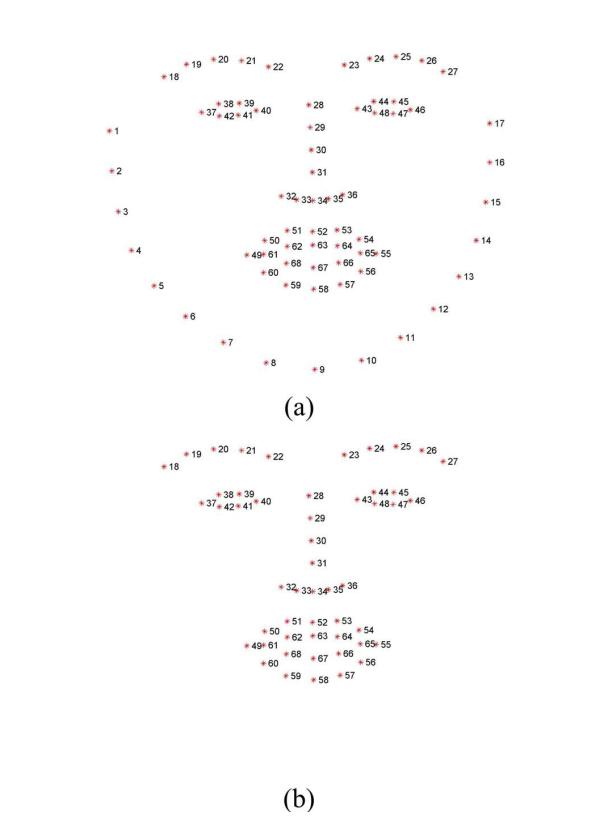
\includegraphics[width=0.8\textwidth]{img/33W.png}
                    \caption{Conjunto de landmarks anotados en el dataset 300W, en la imagen \textit{a} contando el contorno del rostro son un total de 68 landmarks, en la imagen \textit{b} son 51 en total. Imagen extraida de \cite{300W}.}
                    \label{fig:300W}
                \end{figure}
                
                \item \textbf{AFLW}: Se trata de un dataset de $24386$ imágenes \textit{in-the-wild} con un total de 21 landmarks anotados entre las cejas y el mentón, como podemos ver en la imagen \autoref{fig:AFLW}  \cite{AFLW}
                \begin{figure}[!h]
                    \centering
                    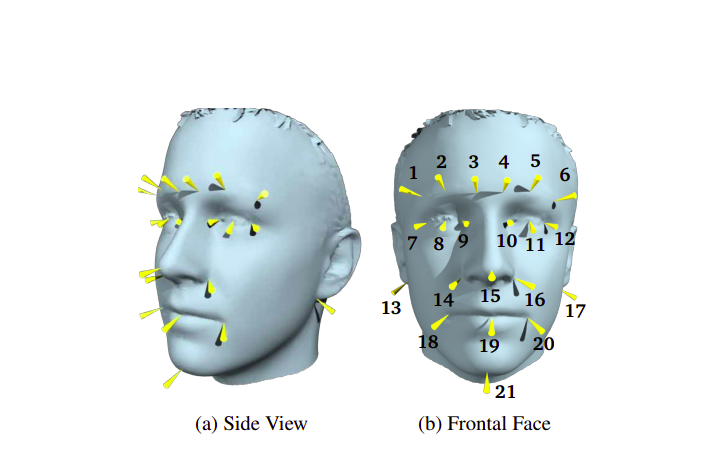
\includegraphics[width=0.8\textwidth]{img/AFLW.png}
                    \caption{Conjunto de landmarks anotados sobre un modelo $3$D que emplea el dataset AFLW. Imagen extraida de \cite{AFLW}.}
                    \label{fig:AFLW}
                \end{figure}
            \end{itemize}
            
            \medskip
            
            \noindent El hecho es que existen actualmente CNN que son capaces de reconocer con un alto grado de precisión estos conjuntos de landmarks marcados por las bases de datos anteriores, lo que nos hace pensar que quizá podría emplearse el conocimiento adquirido por estas redes para reentrenarlas en un proceso de \textit{fine-tuning} sobre una base de datos forense con landmarks anotados por un experto para tratar de resolver el problema de la identificación automática de landmarks. De ahí nace nuestra propuesta, que en cierto modo trata hace como nexo de unión entre las dos vías de investigación.    
\endinput
%------------------------------------------------------------------------------------
% FIN DEL CAPÍTULO. 
%------------------------------------------------------------------------------------

